\section{Feature Selection}
This phase serves a dual purpose. Firstly, since each type of feature (such as MFCC, Chroma, CQT, etc.) can consist of a varying number of individual features,
it is important to determine the optimal number of features for each type to maximize the model's performance.
Secondly, this phase aims to identify which specific features are the most relevant and influential for the classification task.
By doing so, we can enhance the model's efficiency and accuracy by focusing on the features that contribute the most to the classification process.

\subsection{Optimal number of features for each type of feature}
Since each type of feature can consist of a variable number of individual features,
it is necessary to determine the optimal number of features for each type to maximize the model's performance.
To achieve this, a 'One Model per Feature' approach was employed. This involved training a separate model for each type of feature,
varying the number of features used. A set of 12, 20, 30, 40, 60, 70, 90, and 120 features was extracted for each type. For each feature set,
three different models were trained using three classifiers: SVM, Random Forest, and Logistic Regression.\\
Figure \ref{fig:n_feature_per_type} shows the results obtained for each type of feature with the Random Forest model,
as it significantly outperformed the other classifiers.\\
The graph illustrates the F1 scores for different feature types, with varying numbers of features.
The MFCC features consistently achieved the highest F1 scores, peaking around 0.7.
This indicates that MFCC features are particularly effective for the classification task.
Interestingly, the number of features (from 12 to 120) does not drastically affect the performance, suggesting that even a smaller set of MFCC
features can be highly informative.\\
In contrast, the performance of Chroma features is significantly lower compared to MFCC, with F1 scores ranging between 0.3 and 0.4.
This suggests that Chroma features are less effective for this classification task,
and increasing the number of features does not improve the performance substantially.\\
CQT features show moderate performance, with F1 scores around 0.4 to 0.5. The optimal number of features appears to be around 70,
beyond which there is no significant improvement. Similarly, RMS features exhibit a range of F1 scores from 0.4 to 0.5,
with optimal performance achieved with around 70 features.\\
For ZCR, SC, SB, and SR features, the F1 scores generally stabilize around 0.4 to 0.5.
Increasing the number of features beyond 40 does not result in significant performance gains and can even degrade the model's performance.
This suggests that adding too many features, especially those without strong predictive power, can confuse the model and degrade performance.\\
Overall, the optimal number of features varies by type but often falls between 40 and 70.
Adding more features beyond this range does not necessarily improve model performance.
Focusing on the most relevant features and avoiding an excessive number enhances both the efficiency and accuracy of the classification model.
This phase has demonstrated that MFCC features are the most effective for this classification task,
maintaining high performance across different feature counts, while other feature types show varying degrees of effectiveness.

\begin{figure*}[htbp]
    \centering
    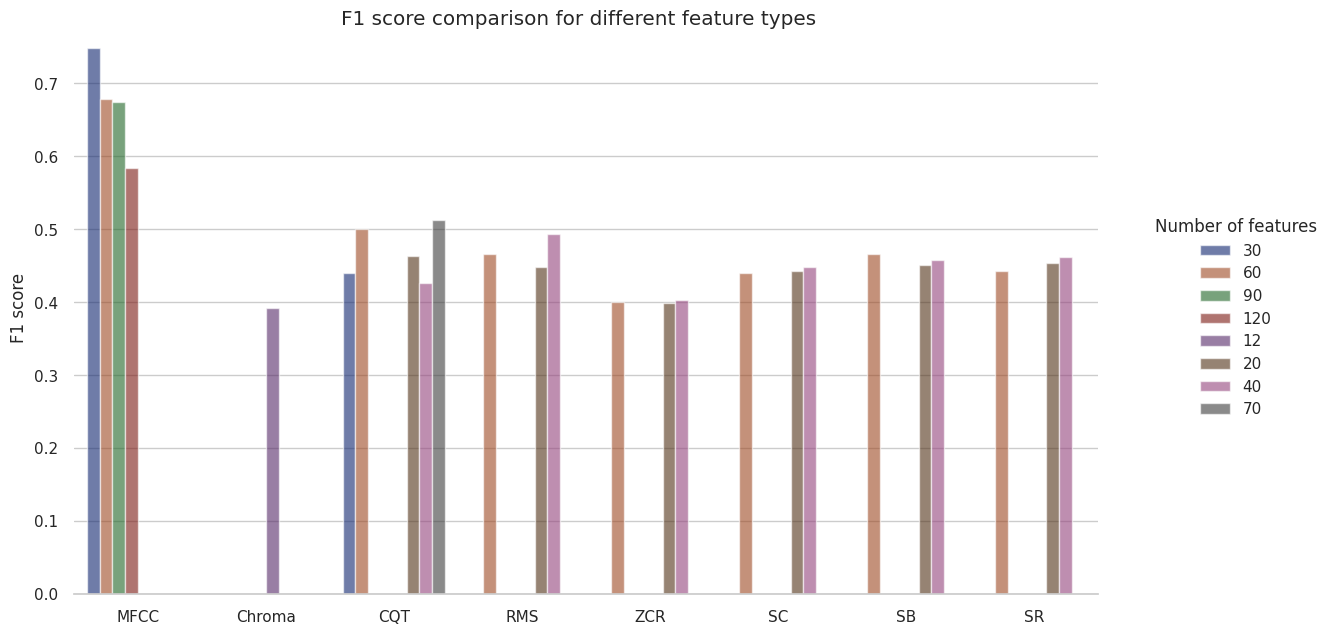
\includegraphics[width=.8\textwidth]{../images/n_feature_per_type.png}
    \caption{F1 score per number of features}
    \label{fig:n_feature_per_type}
\end{figure*}
\noindent
\subsection{Correlation analysis}


\subsection{Results}
